\section{Результаты работы}

Результатом работы является тестирование, разработанных программ на суперкомпьютере Polus. Для тестирования было выбрано количество процессоров равное 1, 2, 3, 4, 5, 6, 7, 8, 9, 10, 20, 40, 60, 80, 100, 120, 140, 160 и входные данные N=\{200, 500, 700, 1000, 1200\}.
Из-за ограничения в 15 минут (900 секунд), для некоторых параметров значения так и не были получены. Эти параметры обозначены темно-синим цветом на диаграмме.


\begin{figure}[H]
    \centering
    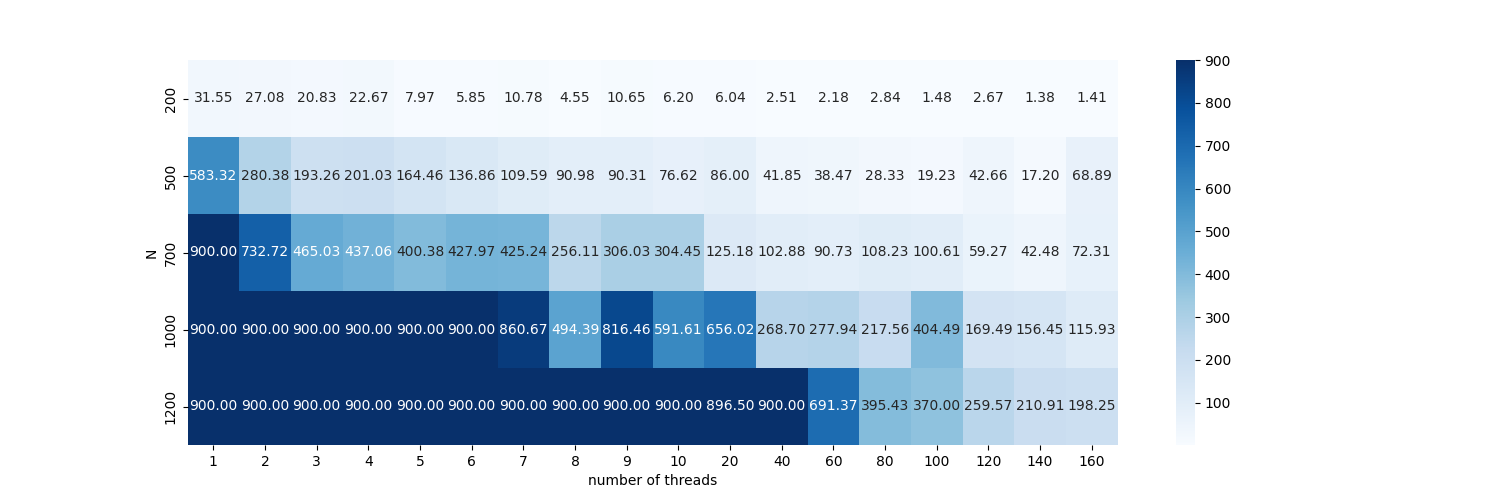
\includegraphics[width=1.\linewidth,center]{openmp_redblack_O0.png}
    \caption{Алгоритм RedBlack3D с флагом \code{O0}}
\end{figure}

\begin{figure}[H]
    \centering
    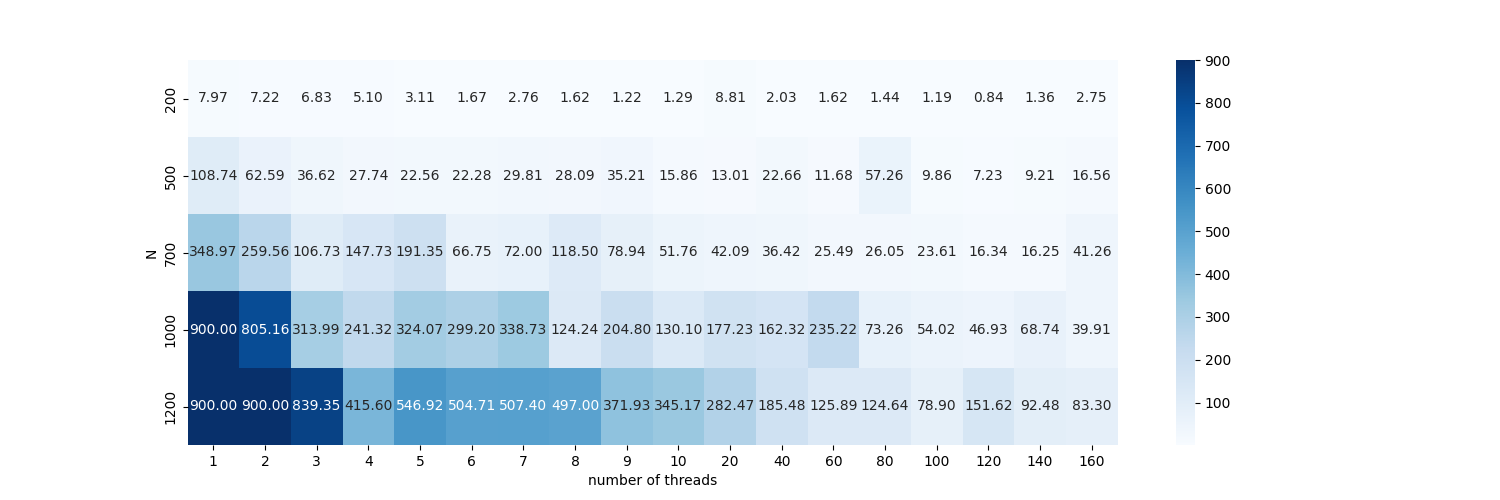
\includegraphics[width=1.\linewidth,center]{openmp_redblack_O2.png}
    \caption{Алгоритм RedBlack3D с флагом \code{O2}}
\end{figure}

\begin{figure}[H]
    \centering
    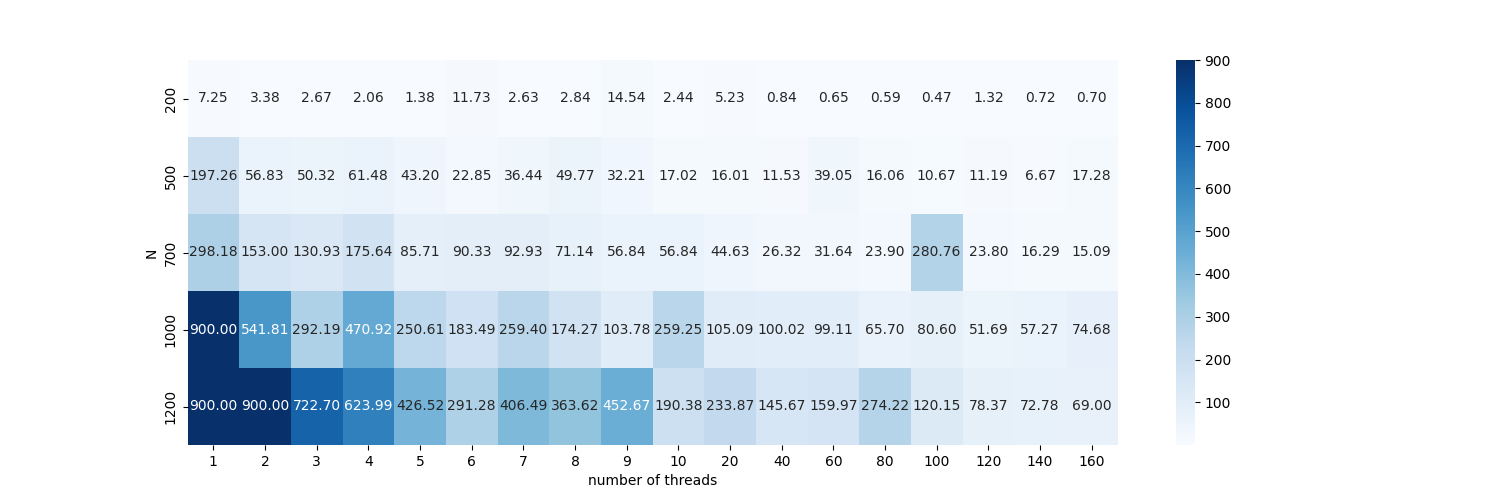
\includegraphics[width=1.\linewidth,center]{openmp_redblack_O3.png}
    \caption{Алгоритм RedBlack3D с флагом \code{O3}}
\end{figure}


\begin{figure}[H]
    \centering
    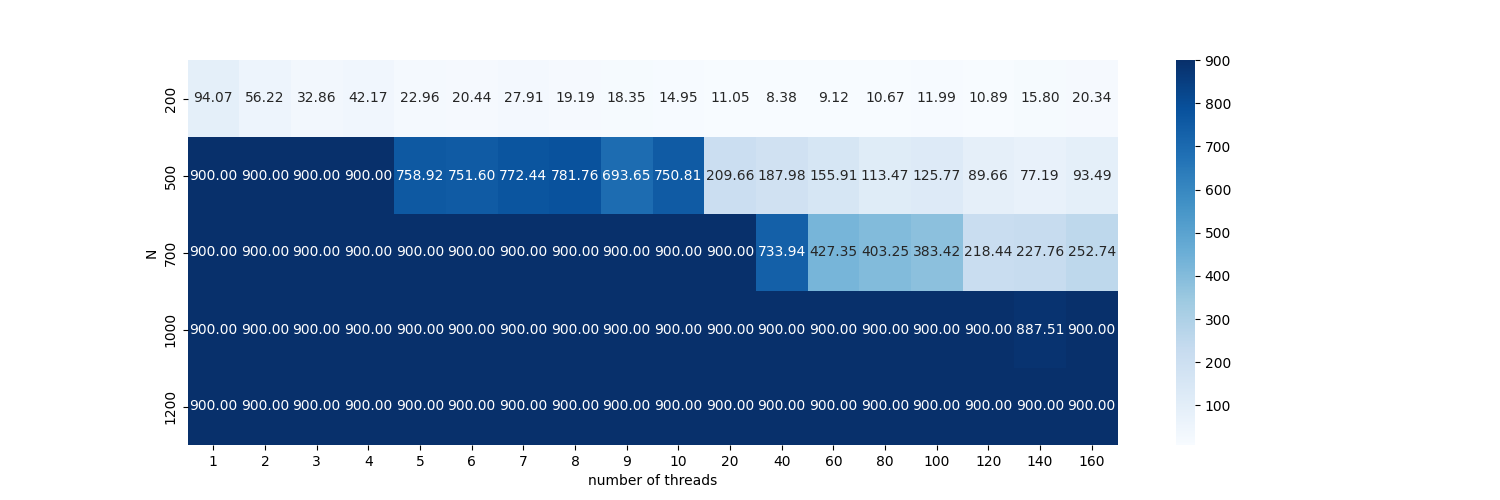
\includegraphics[width=1.\linewidth,center]{openmp_hyperplain_O0.png}
    \caption{Распараллеливание по гиперплоскостям куба с флагом \code{O0}}
\end{figure}

\begin{figure}[H]
    \centering
    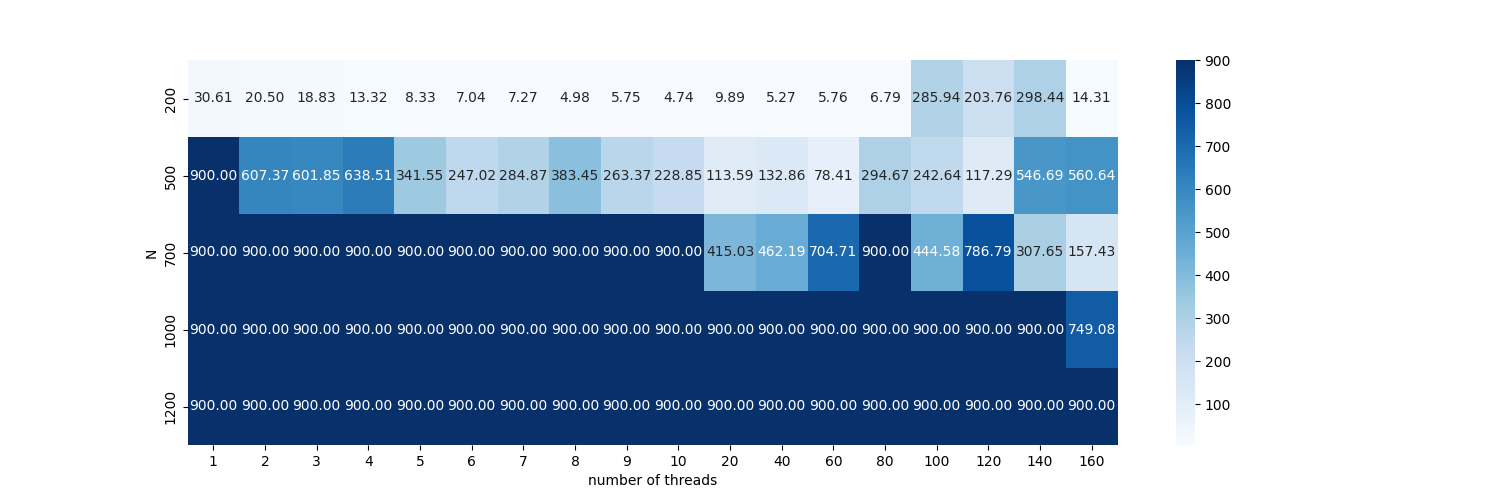
\includegraphics[width=1.\linewidth,center]{openmp_hyperplain_O2.png}
    \caption{Распараллеливание по гиперплоскостям куба с флагом \code{O2}}
\end{figure}

\begin{figure}[H]
    \centering
    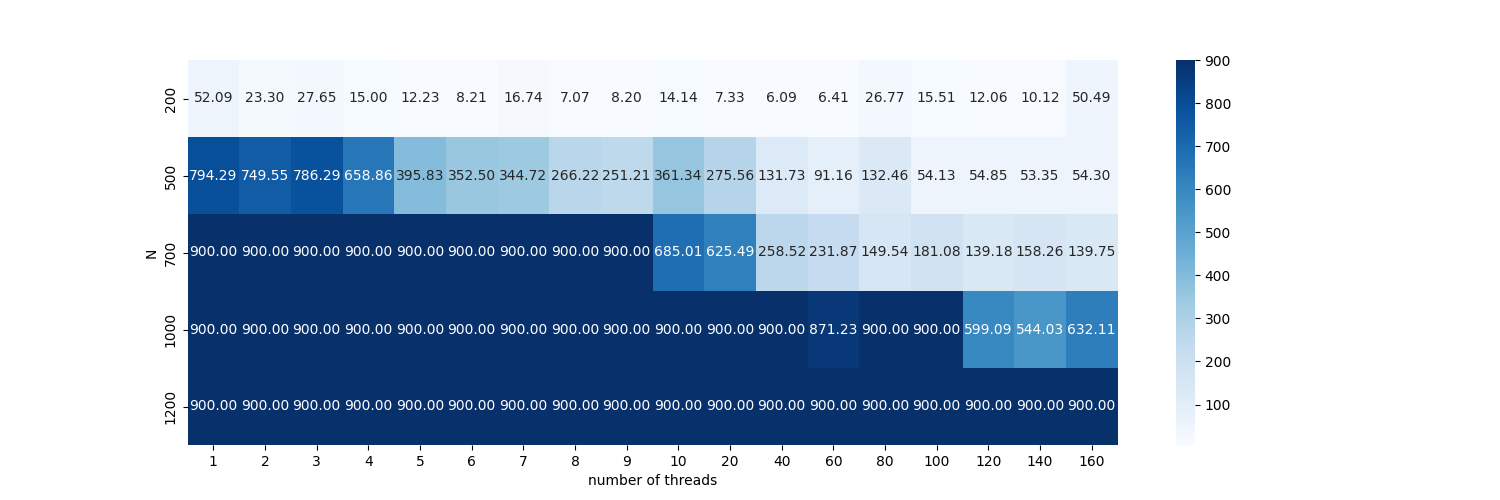
\includegraphics[width=1.\linewidth,center]{openmp_hyperplain_O3.png}
    \caption{Распараллеливание по гиперплоскостям куба с флагом \code{O3}}
\end{figure}


Для визуализации данных была использована библиотека \code{seaborn} для \code{Python 3}.

